\documentclass[12pt,a4paper]{article}
\usepackage[utf8]{inputenc}

\usepackage{multicol}
\usepackage{graphicx}
\usepackage{fancyhdr}
\usepackage{times}
\usepackage{titlesec}
\usepackage{multirow}
\usepackage{lettrine}
\usepackage{hyperref}
\usepackage[top=2cm, bottom=1.5cm, left=2cm, right=2cm]{geometry}
\usepackage[figurename=Fig.,tablename=TAULA]{caption}


\author{\LARGE\sffamily Marc Maldonado Lorca}
\title{\Huge{\sffamily Data Science: Estimación del peso de un cerdo \\
Informe Inicial}}

\date{}

\newcommand\blfootnote[1]{%
  \begingroup
  \renewcommand\thefootnote{}\footnote{#1}%
  \addtocounter{footnote}{-1}%
  \endgroup
}
\renewcommand{\contentsname}{whatever}
\renewcommand{\refname}{Referencias}
%
%\large\bfseries\sffamily
\titleformat{\section}
{\large\sffamily\scshape\bfseries}
{\textbf{\thesection}}{1em}{}

\begin{document}

\fancyhead[LO]{\scriptsize Marc Maldonado Lorca: Estimación del peso de un cerdo}
\fancyhead[RO]{\thepage}
\fancyhead[LE]{\thepage}
\fancyhead[RE]{\scriptsize EE/UAB TFG INFORMÀTICA: Estimación del peso de un cerdo}

\fancyfoot[CO,CE]{}

\fancypagestyle{primerapagina}
{
   \fancyhf{}
   \fancyhead[L]{\scriptsize TFG EN ENGINYERIA INFORMÀTICA, ESCOLA D'ENGINYERIA (EE), UNIVERSITAT AUTÒNOMA DE BARCELONA (UAB)}
   \fancyfoot[C]{\scriptsize ``Septembre'' de 2022, Escola d'Enginyeria (UAB)}
}

%\lhead{\thepage}
%\chead{}
%\rhead{\tiny EE/UAB TFG INFORMÀTICA: Estimación del peso de un cerdo}
%\lhead{ EE/UAB \thepage}
%\lfoot{}
%\cfoot{\tiny{February 2015, Escola d'Enginyeria (UAB)}}
%\rfoot{}
\renewcommand{\headrulewidth}{0pt}
\renewcommand{\footrulewidth}{0pt}
\pagestyle{fancy}

%\thispagestyle{myheadings}


%\vspace*{-1cm}{\scriptsize TFG EN ENGINYERIA INFORMÀTICA, ESCOLA D'ENGINYERIA (EE), UNIVERSITAT AUTÒNOMA DE BARCELONA (UAB)}

\maketitle

\thispagestyle{primerapagina}
%\twocolumn[\begin{@twocolumnfalse}
%\maketitle
%\begin{abstract}
\begin{center}
\parbox{0.915\textwidth}
{\sffamily

}
\bigskip

{\vrule depth 0pt height 0.5pt width 4cm\hspace{7.5pt}%
\raisebox{-3.5pt}{\fontfamily{pzd}\fontencoding{U}\fontseries{m}\fontshape{n}\fontsize{11}{12}\selectfont\char70}%
\hspace{7.5pt}\vrule depth 0pt height 0.5pt width 4cm\relax}

\end{center}

\bigskip
%\end{abstract}


\section{Contexto y objetivos}

\begin{figure}
\caption{Ejemplo de imagen cenital}
\centering
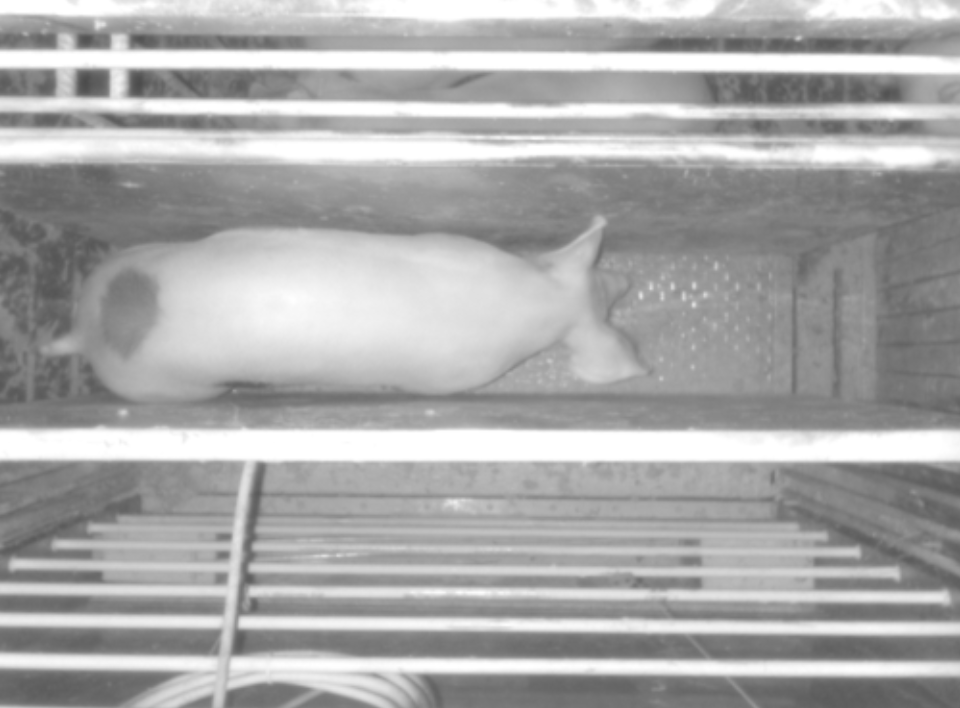
\includegraphics[width=0.5\textwidth]{05-TFG-template-latex/images/foto.png}
\label{foto}
\end{figure}




Desde hace unos años el sector agrario evoluciona junto a las nuevas tecnologías emergentes, lo que se conoce como Smart Farming. Este nuevo concepto aprovecha el potencial de las TIC para abaratar tanto los costes de producción como la eficiencia de las granjas. A partir de esta idea se han ideado nuevos modelos de gestión que van desde los invernaderos inteligentes y la gestión de plagas, hasta la implementación de drones agrícolas que utilizando imágenes aéreas permiten un ahorro significativo de tiempo y mano de obra a la hora de la verificación visual de un cultivo. Ademas no solo es aplicable al cultivo sino que existe una interesante aplicación en el ganado. 



Es por eso que el CVC trabajó en un proyecto de Smart Farming relacionado con la automatización de una granja de cerdos, donde uno de los retos pendientes era estimar el peso de los estos con la motivación de conocer su evolución y prepararlos para dar el peso optimo en el matadero y así obtener la máxima rentabilidad posible. A la hora de entregar un cerdo al matadero su valor depende de lo que se aproxime su peso a loas 120kg, este valor del animal disminuye tanto si su peso es inferior o superior al estándar establecido, es por eso que el control de la evolución de estos animales es tan importante para obtener beneficios. 

\begin{figure}[h]
\caption{Báscula con montaje de la camara}
\centering
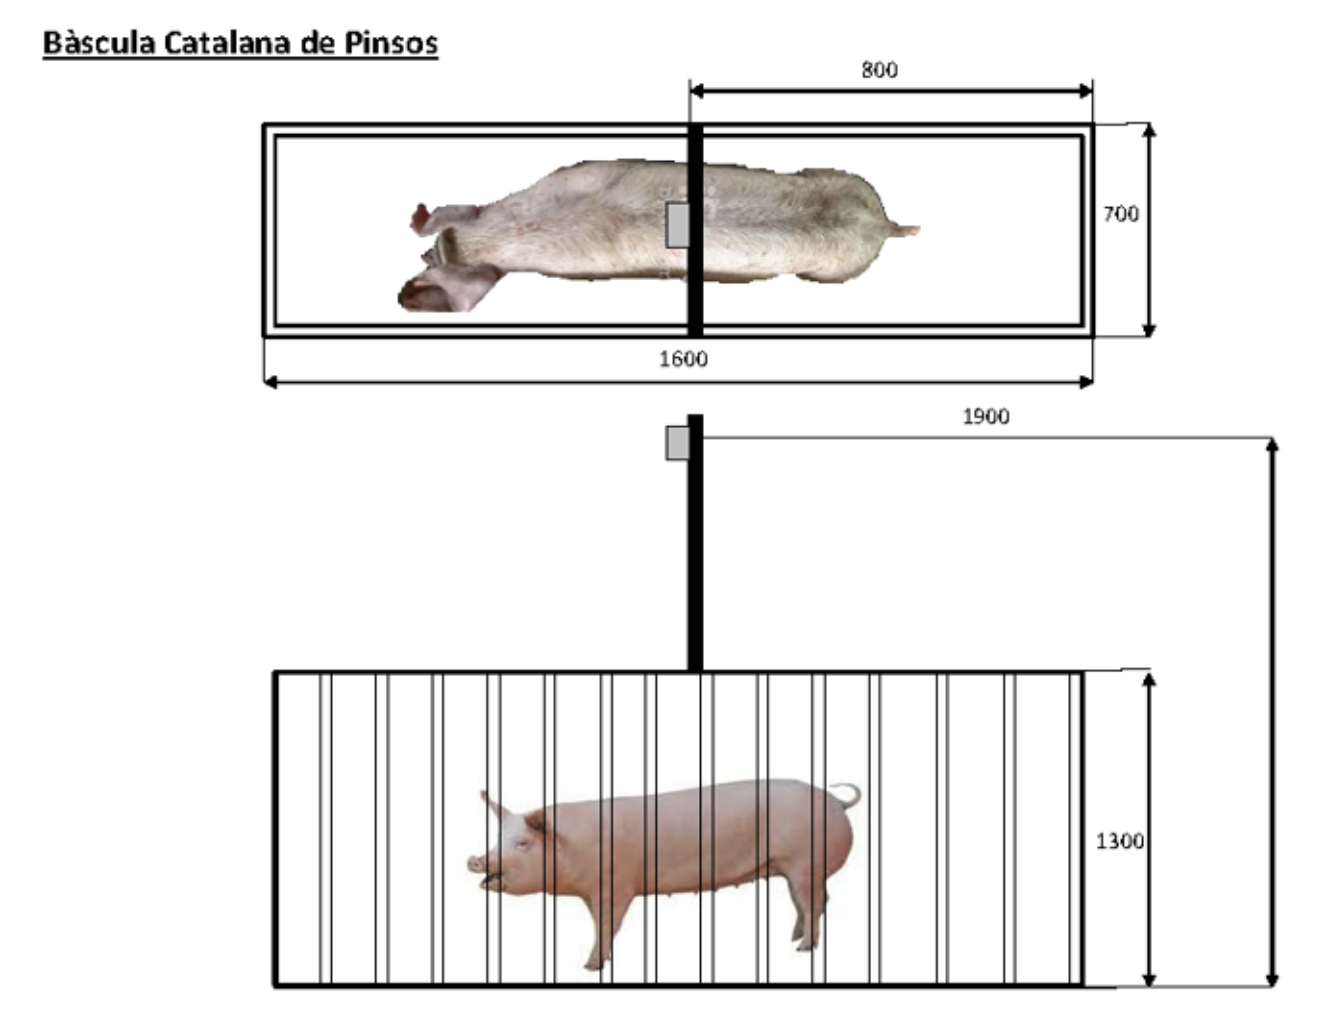
\includegraphics[width=0.6\textwidth]{05-TFG-template-latex/images/montaje.png}
\label{montaje}
\end{figure}
\begin{figure}[h]
\caption{Ejemplo de nube de puntos}
\centering
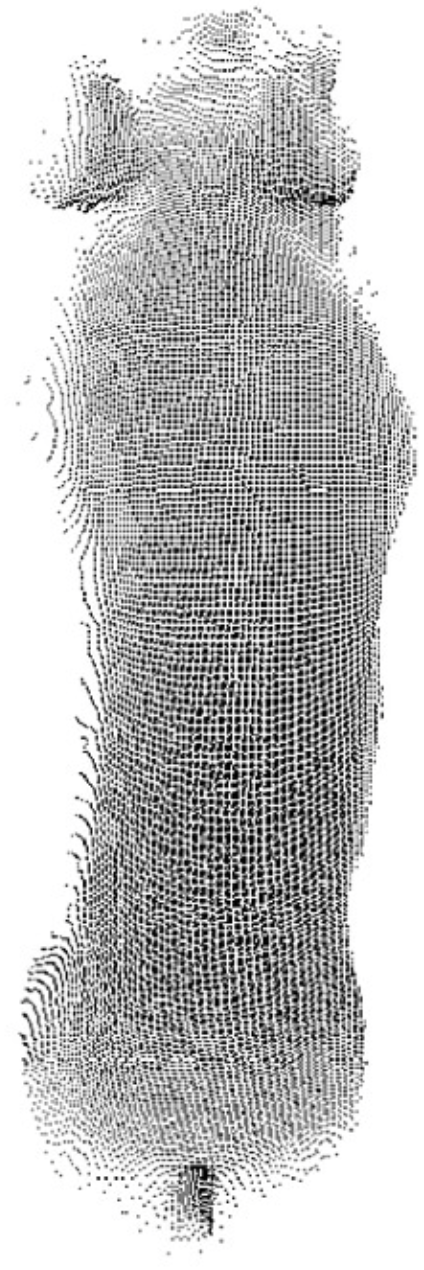
\includegraphics[scale=0.3]{05-TFG-template-latex/images/puntos.png}
\label{puntos}
\end{figure}

El concepto consiste en utilizar una cámara 3D para hacer fotos cenitales de los animales y así eliminar el costoso proceso de utilizar una bascula y agilizar el pesaje aumentando de esta manera el numero de cerdos pesados por unidad de tiempo \cite{sistema}.

Este problema ya ha sido planteado por muchas personas, instituciones y empresas, además de haber sido abordado de distintas maneras y con distintos animales. Se han utilizado imágenes 2D donde se segmenta al cerdo utilizando técnicas de morfología, se construye su esqueleto y con las medidas de este utilizando una regresión se obtiene el peso \cite{Area}. En otro estudio utilizando vacas y una reconstrucción 3D similar a nuestros datos y extrayendo diferentes atributos como la altura, la anchura, el área, etc, consiguen estimar mediante regresión el peso de la vaca entre otros factores\cite{3D}.
También existe otra solución utiliza imágenes de profundidad con las cuales utilizando redes neuronales convolucionales consigue estimar tanto el peso como otras variables biométricas del animal \cite{CNN}.
Finalmente otro estudio mediantes nubes de puntos como las que disponemos y analizando la postura de los cerdos, analizando la relación entre volumen y postura del animal consiguen mediante regresión estimar el peso.


Además de todos estos estudios ya existen productos en el mercado variados con diferentes enfoques.
La empresa PLF AGRITECH \cite{PLF} ha puesto en práctica diferentes tecnologías para el desarrollo de los animales en las granjas inteligentes, aportan una solución al problema de la detección de peso además de un alimentador automático inteligente y un control sobre el impacto medioambiental de estas grajas en términos de aire.
FANCOM \cite{fancom} a parte de tener productos enfocados al crecimiento de otros animales como los pollos o productos destinado al cultivo de hongos también aportan una solución al control del peso de los cerdos con su producto EYEGROW \cite{fancomvideo}. Con una cámara de profundidad en el techo ellos son capaces de segmentar los cerdos individualmente y estimar el peso de ellos simultáneamente para después con la ayuda de un software poder analizar la evolución. Para esta tarea es interesarte leer un articulo de SENSORS \cite{deteccion} que bajo el pretexto de la existencia de pocos datasets de cerdos ofrecen un modelo capaz de identificar a estos en fotos cenitales ademas de identificar la posición de sus distintas partes del cuerpo. Una aplicación similar a la anterior es la de GROSTAT \cite{GroStat}.
\begin{figure}[b]
\caption{Gafas de realidad virtual para la estimación de peso}
\centering
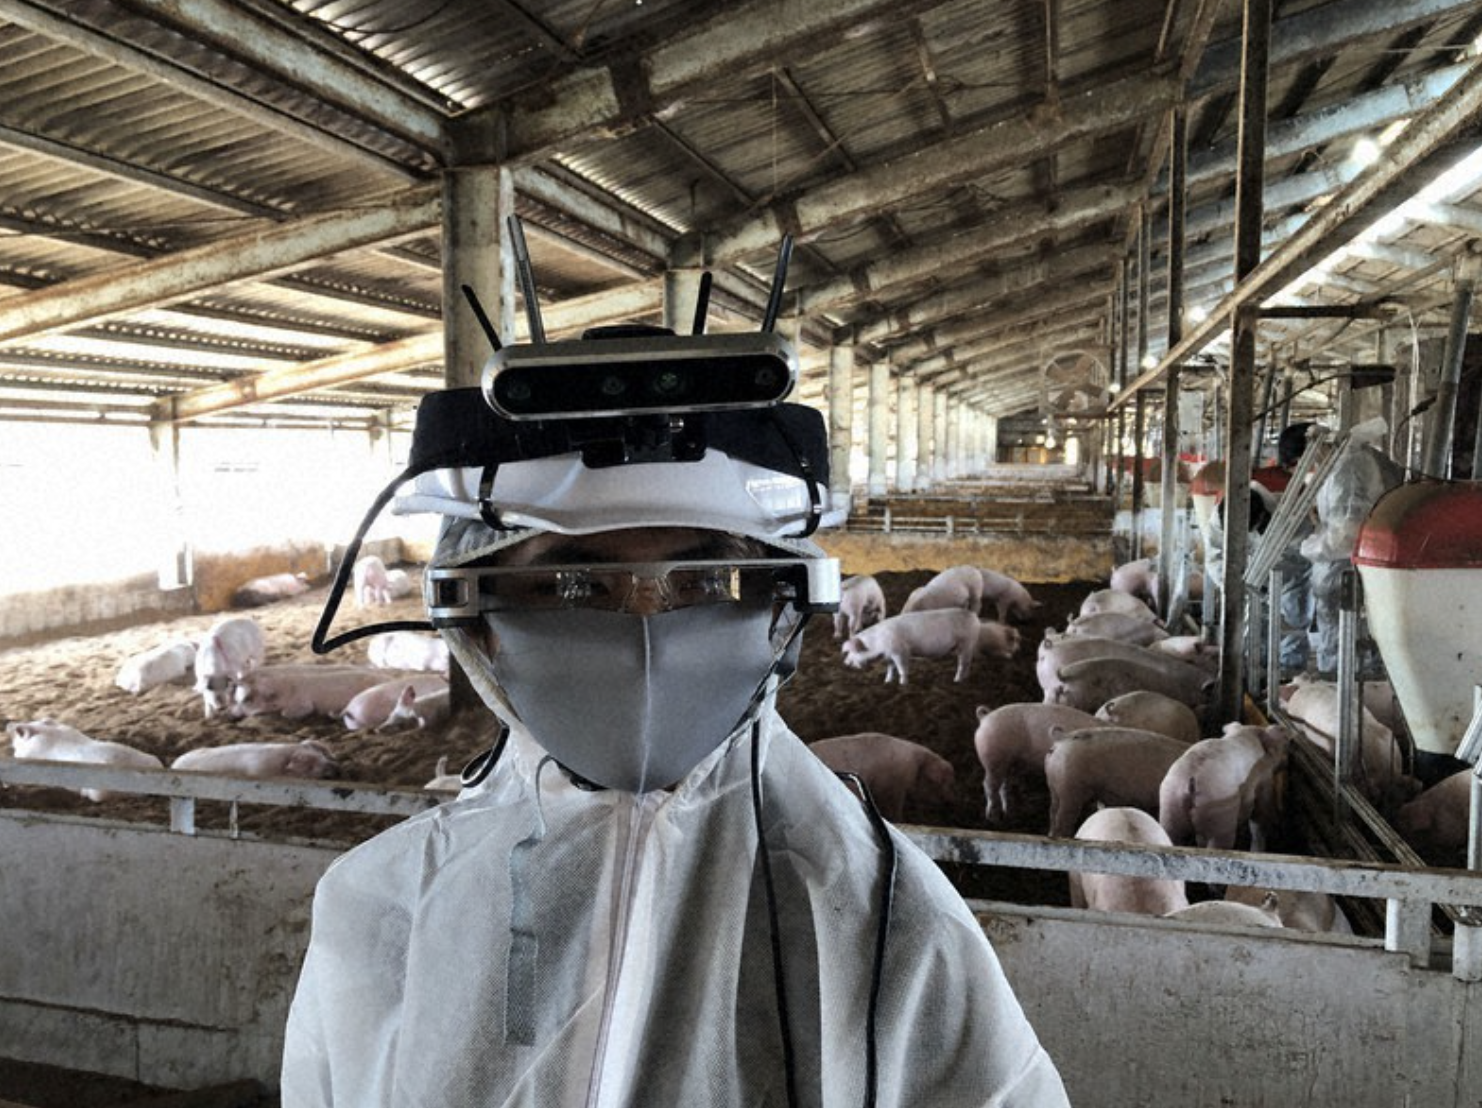
\includegraphics[width=0.5\textwidth]{05-TFG-template-latex/images/gafas.png}
\label{gafas}
\end{figure}
Existe un enfoque diferente en cuanto a la manera de utilizar la cámara, mientras empresas como la anterior deciden colocar la cámara en un lugar fijo, otras empresas optan por la manipulación de la cámara de manera manual, de esta manera se facilitaría la selección del cerdo a pesar. Es el caso de H+L \cite{H+L} o PIGGY CHECK \cite{piggycheck} que mediante cámaras 3D incorporadas en dispositivos móviles consiguen estimar los pesos de los cerdos de manera individual. Existe una solución similar desarrollada por Southwest Japan univ. \cite{japon} pero esta vez la cámara está acoplada a unas GOOGLE glasses \cite{google} como se muestra en la \textbf{Fig \ref{gafas}} de manera que tan solo mirando al cerdo tendríamos la información, aunque todavía no se ha lanzado al mercado.
El peso es un buen indicador de la salud del cerdo pero no es suficiente, DEGREE2ACT \cite{degree} ha desarrollado un gadget para smartphone que mediante una cámara de temperatura nos informa de posibles enfermedades del cerdo, lo cual junto a una estimación del peso podría ser una potente herramienta.

Analizando el contexto y la distribución de nuestra la granja y teniendo en cuenta el recorrido que realizaban los cerdos, se instaló en la báscula tradicional la cámara 3D BASTER BLAZE \cite{camara}, la cual se adapta bien por su resistencia, encargada de recoger el modelo 3D de los cerdos, con imágenes como la que se muestra en la \textbf{Fig \ref{foto}}, y su peso real, todo esto con la ayuda de células fotosensibles que controlarían la entrada individual de cada cerdo a la báscula, además de la instalación de un lector RFID y los respectivos PLC y PC, el montaje se muestra en las \textbf{Fig \ref{montaje}} para procesar y almacenar los datos obtenidos en forma de nube de puntos similar a la \textbf{Fig \ref{puntos}}.


El objetivo real del proyecto extraer el potencial del dataset de las nubes de puntos utilizando modelos de machine learning y encontrar la solución más óptima posible al problema de la estimación del peso de un cerdo utilizando una cámara 3D. En un futuro esta solución combinada a distintas ideas podría ser un producto con bastante potencial.




\section{Metodología}




\begin{table}[!]
\centering
\begin{tabular}{|l|l|l|} 
\hline
Semana~ & 4-6                                           & 6-9                                       \\ 
\hline
        & Estudio del dataset                           & Informe de progreso 1                     \\
        & Eliminación outlayers y substracción de fondo & Conversion de la nube de puntos a malla   \\
        & Visualización de los datos                    & Normalización de los datos                \\ 
\hline
Semana  & 9-10                                          & 10-12                                     \\ 
\hline
        & Separación de train y test                    & Preparación de los parámetros del modelo  \\
        & Búsqueda de redes neuronales                  & Entrenamiento del los modelos             \\ 
\hline
Semana  & 12-14                                         & 14-17                                     \\ 
\hline
        & Informe de progreso 2                         & Preparación Informe final~                \\
        & Análisis de las métricas                      &                                           \\
        & Comparativa con otras soluciones al problema  &                                           \\ 
\hline
Semana  & 17-18                                         &                                           \\ 
\hline
        & Elaboración presentación                      &                                           \\
        & Preparación presentación                      &                                           \\
\hline
\end{tabular}
\caption{Backlog del proyecto}
\label{t:tabla}
\end{table}




Para realizar el trabajo se seguirá la planificación del TFG además de cada semana hacer reuniones individuales con el tutor para así comentar los avances y poder corregir errores. Por eso una metodología ágil se adaptaría perfectamente a este tipo de proyecto. Al ser una sola persona involucrada podemos destacar las diferentes metodologías ágiles que requieres de diferentes roles, por ese motivo decido por optar por Kanban utilizando el software de JIRA, que además proporciona herramientas útiles como el diagrama de gantt.
En la \textbf{TAULA \ref{t:tabla}} y en la \textbf{Fig \ref{gant}} se muestran las tareas que conforman el proyecto repartidas por semanas. Siguiendo esta hoja de ruta y el método Kanban organizaremos las tareas dentro de cuatro apartados en un tablero:

\begin{figure}[!]
\caption{Diagrama de gant}
\centering
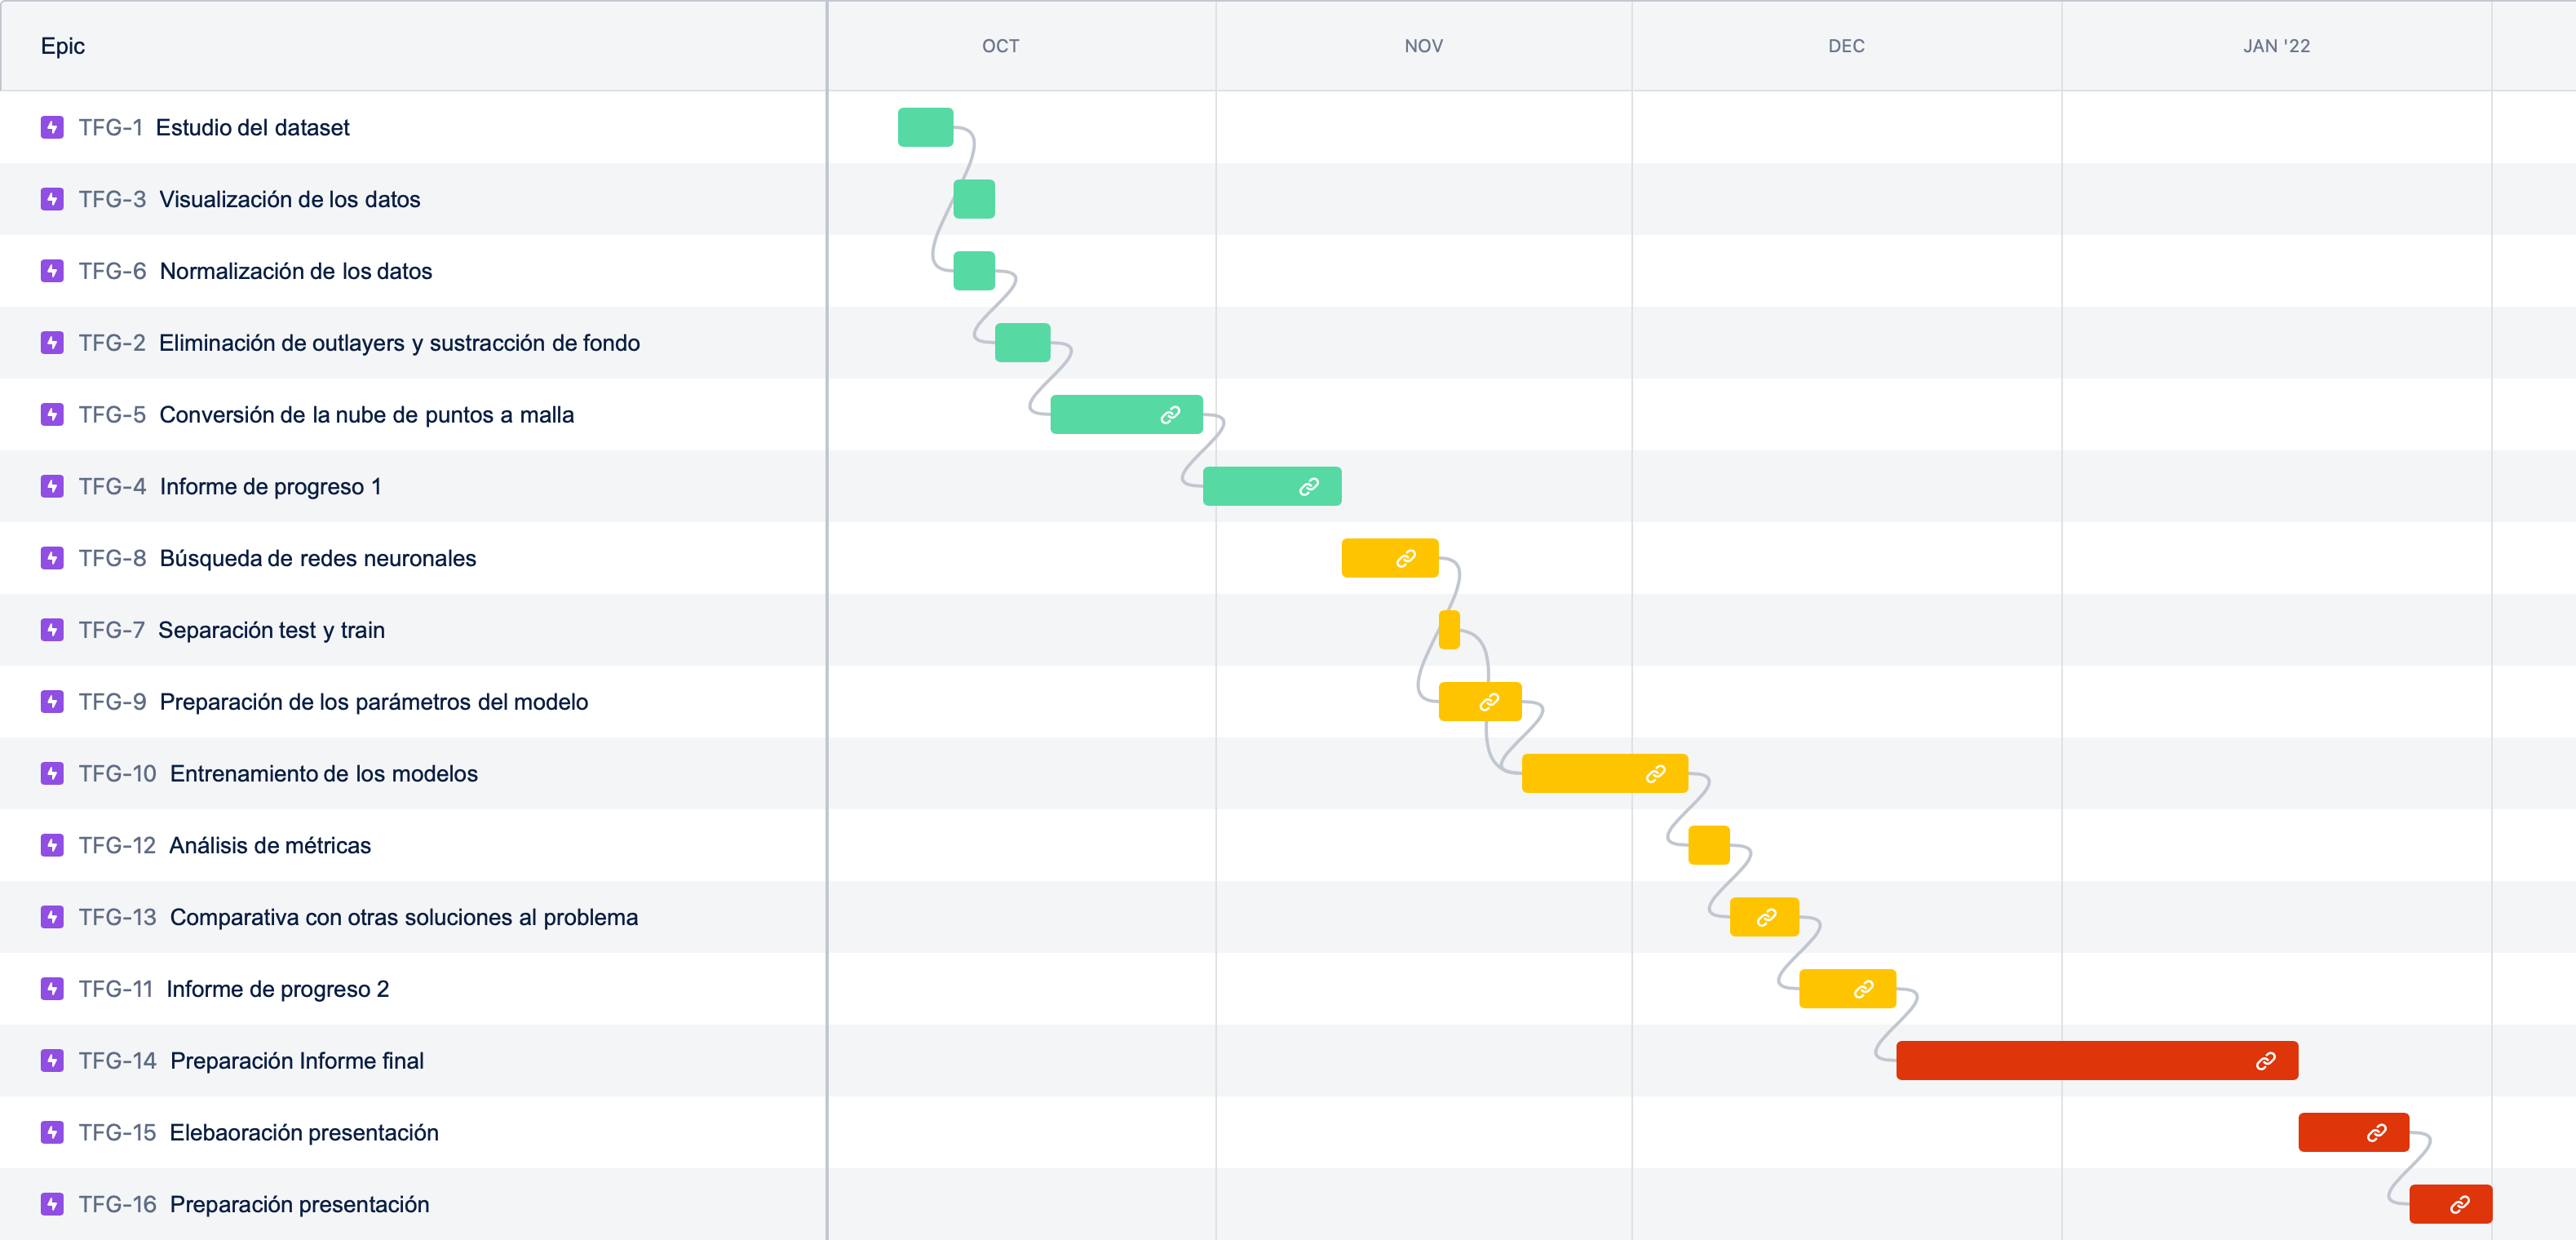
\includegraphics[width=0.8\textwidth]{05-TFG-template-latex/images/gant.png}
\label{gant}
\end{figure}
\begin{itemize}
  \item \textbf{POR HACER: }Aquí se colocarán todas las tareas que todavía no se han empezado a hacer, de aquí solo se podrán mover a la columna EN PROGRESO.
  \item \textbf{EN PROGRESO: }Aquí se colocarán las tareas que se encuentran en desarrollo, solo se podrán mover hacia el estado EN REVISIÓN.
  \item \textbf{EN REVISIÓN: }Esta columna contiene las tareas acabadas pendientes de revisión por el tutor, en el caso de completarse satisfactoriamente se moverán a HECHO, en el caso contrario volverán a EN PROGRESO.
  \item \textbf{HECHO: }Este apartado contendrá las tareas finalizadas.
\end{itemize}


Con los apartados anteriores sería suficiente para monitorizar el flujo de trabajo y obtener el flujo de rendimiento.



\section{Planificación}




Como hemos comentado, la motivación es estimar los pesos de los cerdos utilizando herramientas de machine learning así que la idea principal será transformar estos objetos manipulables para diferentes CNN o GNN, de esta manera distinguimos 2 grandes fases, la preparación de los datos, y la parte del modelo. Lo primero será limpiar nuestros datos tratando de eliminar los puntos que no pertenecen al cerdo, así que mediante morfología trataremos con las imágenes segmentar al animal eliminando así todos los puntos pertenecientes al fondo. Lo siguiente será construir una malla de la superficie del cerdo que nuestra GNN interpretará como un grafo. Una vez con los datos listos para entrenar se procede a la construcción del modelo, para ello se experimentará con diferentes arquitecturas de redes y se modificarán sus parámetros internos para de esta manera conseguir la solución que minimice el error (MSE), ya que nuestro objetivo es acercarnos lo máximo al peso real. Esta es una primera idea de como se implementara la solución, es probable que aparezcan cambios durante el desarrollo.

\begin{thebibliography}{5}

\bibitem{sistema}
    AHDB Pork \emph{"Pigs 2022 - Pig weighing systems"} [Online 30/9/2021]
    \url{https://www.youtube.com/watch?v=3CuLNYhFOjk}
    
\bibitem{camara}
    Basler \emph{"Basler blaze"} [Online 30/9/2021]
    \url{https://www.baslerweb.com/en/products/cameras/3d-cameras/basler-blaze/}

\bibitem{Area}
    K. Kollis, C.S. Phang, T.M. Banhazi and S.J. Searle \emph{"Weight estimation using image analysis and
    statistical modelling: A preliminary study"} [Online 30/9/2021]
    \url{https://www.researchgate.net/publication/236886740_Weight_Estimation_Using_Image_Analysis_and_Statistical_Modelling_A_Preliminary_Study}
\bibitem{3D}
    Dorota Anglart \emph{"Automatic estimation of body weight and body condition score in dairy cows using 3D imaging technique"} [Online 30/9/2021]
    \url{https://stud.epsilon.slu.se/6355/1/anglart_d_140114.pdf}
\bibitem{CNN}
    Jianlong Zhang, Yanrong Zhuang, Hengyi Ji, and Guanghui Teng \emph{"Pig Weight and Body Size Estimation Using a Multiple Output Regression Convolutional Neural Network: A Fast and Fully Automatic Method"} [Online 30/9/2021]
    \url{https://www.researchgate.net/publication/352102505_Pig_Weight_and_Body_Size_Estimation_Using_a_Multiple_Output_Regression_Convolutional_Neural_Network_A_Fast_and_Fully_Automatic_Method}
    
\bibitem{PLF}
    PLF Agritech \emph{"PLF Agritech"} [Online 30/9/2021]
    \url{http://plfag.com/technologies/}
    
\bibitem{fancom}
    Fancom \emph{"Fancom"} [Online 30/9/2021]
    \url{https://www.fancom.com}

\bibitem{fancomvideo}
    Fancom BV \emph{"eYeGrow - Weight monitor for finishers"} [Online 30/9/2021]
    \url{https://www.youtube.com/watch?v=CSuWWgY43PA}    

\bibitem{deteccion}
    Eric T. Psota, Mateusz Mittek, Lance Pérez and Ty B Schmidt \emph{"Multi-Pig Part Detection and Association with a Fully Convolutional Network"} [Online 30/9/2021]
    \url{https://www.researchgate.net/publication/352102505_Pig_Weight_and_Body_Size_Estimation_Using_a_Multiple_Output_Regression_Convolutional_Neural_Network_A_Fast_and_Fully_Automatic_Method}
    
\bibitem{GroStat}
    GroStat \emph{"GROWTH SENSOR"} [Online 30/9/2021]
    \url{http://grostat.com/growth_sensor.php#prettyPhoto}

\bibitem{H+L}
    H+L \emph{"optiSCAN"} [Online 30/9/2021]
    \url{https://hl-agrar.de/en_gb/optiscan/}

\bibitem{piggycheck}
    Agro Napló \emph{"Piggy Check – weigh pigs with your tablet PC"} [Online 30/9/2021]
    \url{https://www.agronaplo.hu/nagyvilag/piggy-check-weigh-pigs-with-your-tablet-pc}

\bibitem{japon}
    The Mainichi \emph{"Southwest Japan univ. develops smart glasses to visually estimate pigs' weight"} [Online 30/9/2021]
    \url{https://mainichi.jp/english/articles/20210601/p2a/00m/0na/007000c}

\bibitem{google}
    Glass \emph{"Glass"} [Online 30/9/2021]
    \url{https://www.google.com/glass/start/}
    
\bibitem{degree}
    degree2act \emph{"degree2act"} [Online 30/9/2021]
    \url{https://www.degree2act.com/}

\end{thebibliography}



\setcounter{section}{1}

\blfootnote{$\bullet$ E-mail de contacte: maldonadolorcamarc@gmail.com}
\blfootnote{$\bullet$ Menció realitzada: Computació}
\blfootnote{$\bullet$ Treball tutoritzat per: Coen Antens (CVC)}
\blfootnote{$\bullet$ Curs 2021/22}
\end{document}

